% Options for packages loaded elsewhere
\PassOptionsToPackage{unicode}{hyperref}
\PassOptionsToPackage{hyphens}{url}
%
\documentclass[
]{book}
\usepackage{amsmath,amssymb}
\usepackage{lmodern}
\usepackage{iftex}
\ifPDFTeX
  \usepackage[T1]{fontenc}
  \usepackage[utf8]{inputenc}
  \usepackage{textcomp} % provide euro and other symbols
\else % if luatex or xetex
  \usepackage{unicode-math}
  \defaultfontfeatures{Scale=MatchLowercase}
  \defaultfontfeatures[\rmfamily]{Ligatures=TeX,Scale=1}
\fi
% Use upquote if available, for straight quotes in verbatim environments
\IfFileExists{upquote.sty}{\usepackage{upquote}}{}
\IfFileExists{microtype.sty}{% use microtype if available
  \usepackage[]{microtype}
  \UseMicrotypeSet[protrusion]{basicmath} % disable protrusion for tt fonts
}{}
\makeatletter
\@ifundefined{KOMAClassName}{% if non-KOMA class
  \IfFileExists{parskip.sty}{%
    \usepackage{parskip}
  }{% else
    \setlength{\parindent}{0pt}
    \setlength{\parskip}{6pt plus 2pt minus 1pt}}
}{% if KOMA class
  \KOMAoptions{parskip=half}}
\makeatother
\usepackage{xcolor}
\IfFileExists{xurl.sty}{\usepackage{xurl}}{} % add URL line breaks if available
\IfFileExists{bookmark.sty}{\usepackage{bookmark}}{\usepackage{hyperref}}
\hypersetup{
  pdftitle={Data Sovereignty and Open Data in Environmental Sciences},
  hidelinks,
  pdfcreator={LaTeX via pandoc}}
\urlstyle{same} % disable monospaced font for URLs
\usepackage{longtable,booktabs,array}
\usepackage{calc} % for calculating minipage widths
% Correct order of tables after \paragraph or \subparagraph
\usepackage{etoolbox}
\makeatletter
\patchcmd\longtable{\par}{\if@noskipsec\mbox{}\fi\par}{}{}
\makeatother
% Allow footnotes in longtable head/foot
\IfFileExists{footnotehyper.sty}{\usepackage{footnotehyper}}{\usepackage{footnote}}
\makesavenoteenv{longtable}
\usepackage{graphicx}
\makeatletter
\def\maxwidth{\ifdim\Gin@nat@width>\linewidth\linewidth\else\Gin@nat@width\fi}
\def\maxheight{\ifdim\Gin@nat@height>\textheight\textheight\else\Gin@nat@height\fi}
\makeatother
% Scale images if necessary, so that they will not overflow the page
% margins by default, and it is still possible to overwrite the defaults
% using explicit options in \includegraphics[width, height, ...]{}
\setkeys{Gin}{width=\maxwidth,height=\maxheight,keepaspectratio}
% Set default figure placement to htbp
\makeatletter
\def\fps@figure{htbp}
\makeatother
\setlength{\emergencystretch}{3em} % prevent overfull lines
\providecommand{\tightlist}{%
  \setlength{\itemsep}{0pt}\setlength{\parskip}{0pt}}
\setcounter{secnumdepth}{5}
\usepackage{booktabs}
\ifLuaTeX
  \usepackage{selnolig}  % disable illegal ligatures
\fi
\usepackage[]{natbib}
\bibliographystyle{plainnat}

\title{Data Sovereignty and Open Data in Environmental Sciences}
\author{}
\date{\vspace{-2.5em}2022-05-26}

\begin{document}
\maketitle

{
\setcounter{tocdepth}{1}
\tableofcontents
}
\hypertarget{about-this-book}{%
\chapter*{About this book}\label{about-this-book}}
\addcontentsline{toc}{chapter}{About this book}

This is an evolving reading list geared towards understanding the ethical concerns and best practices of data collection, management, and analysis especially as it pertains to working with Indigenous peoples and environmental science and management. Here, you'll find an overview of data sovereignty networks, and a collection of podcasts, seminars, books and peer-reviewed papers. If you're aware of a resource that would fit in well, please share!

This reading list reflects the continuous development of learning materials at the Arctic Data Center (ADC) and National Center for Ecological Analysis and Synthesis (NCEAS) to support researchers and practitioners to understand, adopt, and apply ethical open science practices. In bringing these materials together we recognize that many individuals have contributed to their development. The primary authors are listed in the citation below, with additional contributors recognized for their role in guiding the development of the document or by developing previous iterations.

\textbf{Citation}: Phoebe Racine \& Natasha Haycock-Chavez. 2022. Data Sovereignty and Open Data in Environmental Sciences

\textbf{Additional contributors}: Nākoa Farrant, Ben Halpern, Matt Jones

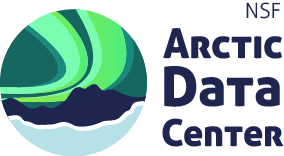
\includegraphics{images/adc_logo.png}
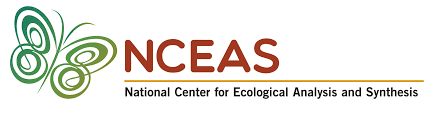
\includegraphics{images/nceas.png}

\hypertarget{land-acknowledgement}{%
\section*{Land Acknowledgement}\label{land-acknowledgement}}
\addcontentsline{toc}{section}{Land Acknowledgement}

This book was created on unceded Chumash ancestral lands in gratitude and solidarity with all our relations. We are committed to learning about how to implement Indigenous Data Sovereignty within our own institutions and in the trainings that Arctic Data Centers offers the Arctic research community.

\hypertarget{ids-indigenous-data-sovereignty-frameworks-networks}{%
\chapter{IDS (Indigenous Data Sovereignty) Frameworks \& Networks}\label{ids-indigenous-data-sovereignty-frameworks-networks}}

International and nation-state networks of practitioners and researchers have formed to share and develop resources and training on data management.

\hypertarget{overview-of-indigenous-data-sovereignty-networks}{%
\section*{Overview of Indigenous data sovereignty networks}\label{overview-of-indigenous-data-sovereignty-networks}}
\addcontentsline{toc}{section}{Overview of Indigenous data sovereignty networks}

\begin{itemize}
\tightlist
\item
  International Groups

  \begin{itemize}
  \tightlist
  \item
    The Global Indigenous Data Alliance \href{https://www.gida-global.org/}{GIDA}
  \item
    International Indigenous Data Sovereignty Interest Group: Research Data Alliance (\href{https://www.rd-alliance.org/groups/international-indigenous-data-sovereignty-ig}{RDA})
  \end{itemize}
\item
  Anglo-settler state data sovereignty networks

  \begin{itemize}
  \tightlist
  \item
    \href{https://usindigenousdata.org/}{U.S. Indigenous Data Sovereignty Network}
  \item
    \href{https://www.temanararaunga.maori.nz/}{Te Mana Raraunga} -- Māori Data Sovereignty Network
  \item
    \href{https://www.maiamnayriwingara.org/}{The Maiam nayri Wingara Indigneous Data Sovereignty Collective}
  \end{itemize}
\end{itemize}

\hypertarget{the-global-indigenous-data-alliance-gida}{%
\subsubsection*{\texorpdfstring{The Global Indigenous Data Alliance (\href{https://www.gida-global.org/}{GIDA})}{The Global Indigenous Data Alliance (GIDA)}}\label{the-global-indigenous-data-alliance-gida}}
\addcontentsline{toc}{subsubsection}{The Global Indigenous Data Alliance (\href{https://www.gida-global.org/}{GIDA})}

Share frameworks, tools, and processes to help guide the practice of Indigenous Data Sovereignty around the globe

\begin{itemize}
\tightlist
\item
  Held a 2019 UN Workshop on data sovereignty
\end{itemize}

\hypertarget{research-data-alliance-rda}{%
\subsubsection*{\texorpdfstring{Research Data Alliance (\href{https://www.rd-alliance.org/groups/international-indigenous-data-sovereignty-ig}{RDA})}{Research Data Alliance (RDA)}}\label{research-data-alliance-rda}}
\addcontentsline{toc}{subsubsection}{Research Data Alliance (\href{https://www.rd-alliance.org/groups/international-indigenous-data-sovereignty-ig}{RDA})}

Building the social and technical bridges to enable open sharing and re-use of data

\begin{itemize}
\tightlist
\item
  Membership for individuals and organizations
\end{itemize}

\hypertarget{indigenous-statistics-the-importance-of-data-to-indigenous-communities}{%
\chapter{Indigenous Statistics: The Importance of Data to Indigenous Communities}\label{indigenous-statistics-the-importance-of-data-to-indigenous-communities}}

\hypertarget{walter-maggie-and-chris-andersen.-indigenous-statistics-a-quantitative-research-methodology.-routledge-2016.}{%
\subsection*{\texorpdfstring{Walter, Maggie, and Chris Andersen. \href{https://www.taylorfrancis.com/books/mono/10.4324/9781315426570/indigenous-statistics-maggie-walter-chris-andersen}{Indigenous statistics}: A quantitative research methodology. Routledge, 2016.}{Walter, Maggie, and Chris Andersen. Indigenous statistics: A quantitative research methodology. Routledge, 2016.}}\label{walter-maggie-and-chris-andersen.-indigenous-statistics-a-quantitative-research-methodology.-routledge-2016.}}
\addcontentsline{toc}{subsection}{Walter, Maggie, and Chris Andersen. \href{https://www.taylorfrancis.com/books/mono/10.4324/9781315426570/indigenous-statistics-maggie-walter-chris-andersen}{Indigenous statistics}: A quantitative research methodology. Routledge, 2016.}

Quantitative data on Indigenous peoples have been taken for granted as straightforward, transparent numbers. With a focus on population statistics and examples from Indigenous peoples in the United States, Australia, and Canada, Maggie Walter and Chris Anderson suggest a paradigm for Indigenous quantitative methods. This book is especially useful in understanding the systemic nature of data inequality in the context of Indigenous communities, why data is important, and how we might improve upon these systems.

\hypertarget{noisecat-julian.-census-powwow.-snap-judgment.-june-2021.}{%
\subsection*{\texorpdfstring{Noisecat, Julian. ``\href{https://open.spotify.com/episode/28040mhUkpvUtas8bd6rmE?si=e0j9BvQ5R9m3e0AGbZajSw}{Census Powwow}.'' Snap Judgment. June 2021.}{Noisecat, Julian. ``Census Powwow.'' Snap Judgment. June 2021.}}\label{noisecat-julian.-census-powwow.-snap-judgment.-june-2021.}}
\addcontentsline{toc}{subsection}{Noisecat, Julian. ``\href{https://open.spotify.com/episode/28040mhUkpvUtas8bd6rmE?si=e0j9BvQ5R9m3e0AGbZajSw}{Census Powwow}.'' Snap Judgment. June 2021.}

Journalist Julian Noisecat follows Cheyanne Brady, a member of the Mandan Hidatsa Arikara Nation, as she works to count everyone on her reservation for the US 2020 Census. This podcast details the complicated relationship tribal nations have with the US Census. Through storytelling, the listener can get a sense of the important role data has in shaping indigenous outcomes.

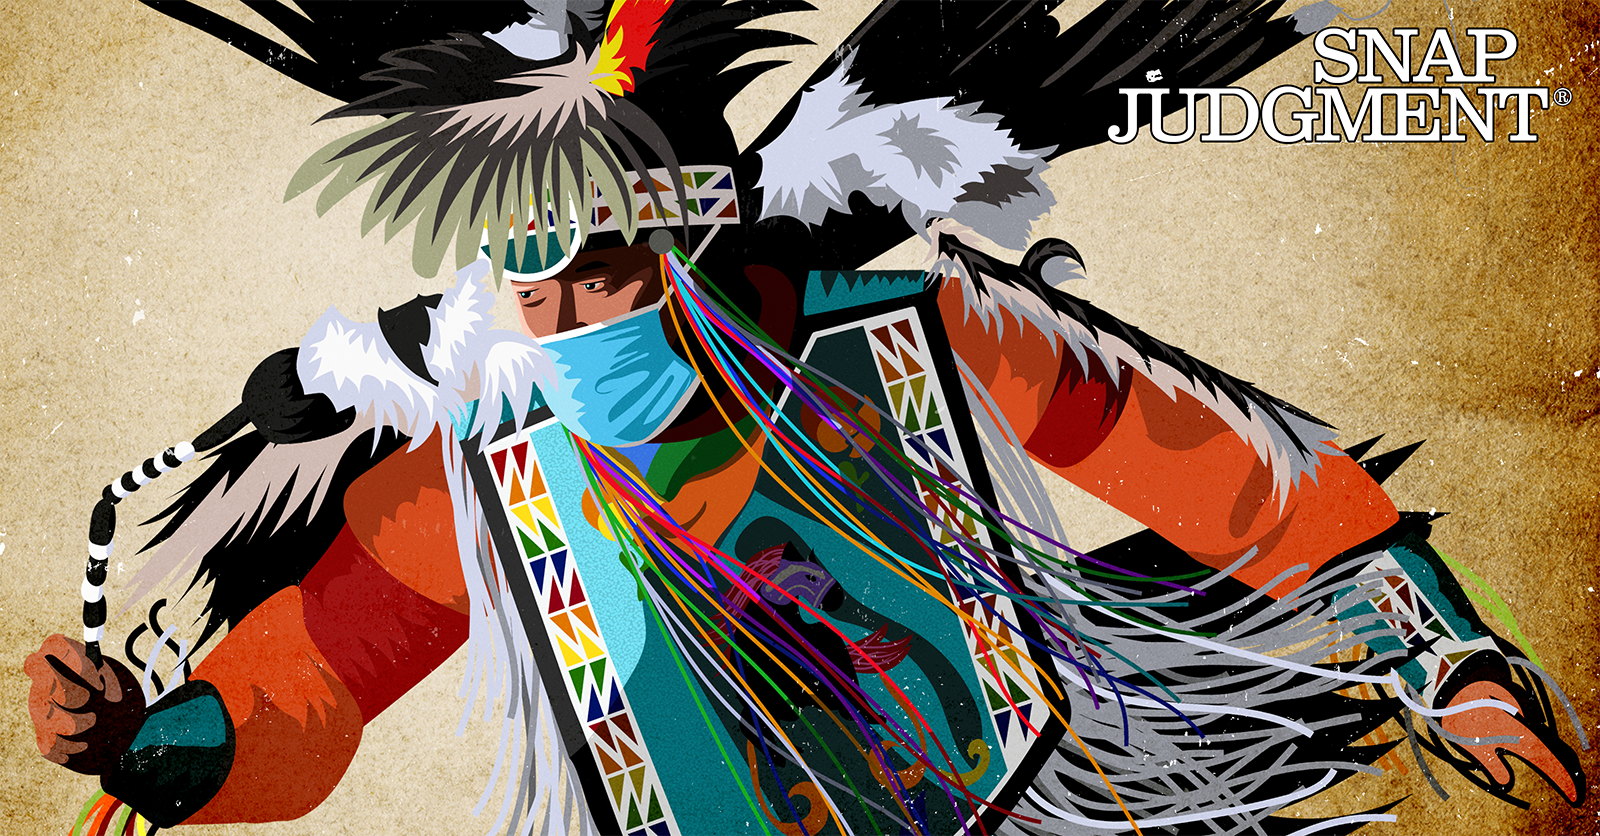
\includegraphics{images/CensusPowwow.png}

\hypertarget{data-sovereignty-and-governance}{%
\chapter{Data Sovereignty and Governance}\label{data-sovereignty-and-governance}}

Data collection, analysis and sharing is couched in historic inequities, some of which Open Data can exacerbate. \textbf{Data sovereignty} maintains that data collected about a community should be managed in a way that is consistent with the laws, practices and customs of that community (\href{https://static1.squarespace.com/static/5d2633cb0ef5e4000134fa02/t/5d7a7610da91c0143184a9d1/1568306712324/Indigenous\%2BData\%2BSovereignty\%2BBook.pdf}{Snipp 2016}, pg. 39). Data Sovereignty addresses aspects of data inequality, and may place limits on what data can be shared and by whom. \textbf{Data governance} is ``the power to decide how and when Indigenous data are gathered, analysed, accessed and used'' (Walter et al.~2018, p.~3).

For a background on these terms see \href{https://datascience.codata.org/articles/10.5334/dsj-2019-031/}{Carroll, Rodriguez-Lonebear, and Martinez 2019}.

\hypertarget{data-sovereignty}{%
\section{Data Sovereignty}\label{data-sovereignty}}

\hypertarget{kukutai-tahu-and-john-taylor.-indigenous-data-sovereignty-toward-an-agenda.-anu-press-2016.}{%
\subsubsection*{\texorpdfstring{Kukutai, Tahu, and John Taylor. \href{https://static1.squarespace.com/static/5d2633cb0ef5e4000134fa02/t/5d7a7610da91c0143184a9d1/1568306712324/Indigenous\%2BData\%2BSovereignty\%2BBook.pdf}{Indigenous Data Sovereignty}: Toward an Agenda. ANU Press, 2016.}{Kukutai, Tahu, and John Taylor. Indigenous Data Sovereignty: Toward an Agenda. ANU Press, 2016.}}\label{kukutai-tahu-and-john-taylor.-indigenous-data-sovereignty-toward-an-agenda.-anu-press-2016.}}
\addcontentsline{toc}{subsubsection}{Kukutai, Tahu, and John Taylor. \href{https://static1.squarespace.com/static/5d2633cb0ef5e4000134fa02/t/5d7a7610da91c0143184a9d1/1568306712324/Indigenous\%2BData\%2BSovereignty\%2BBook.pdf}{Indigenous Data Sovereignty}: Toward an Agenda. ANU Press, 2016.}

\emph{Indigenous Data Sovereignty} is a book published in 2016 and is a collaboration between Indigenous scholars from Anglo-Settler states (CANSUZ), Australia, Aotearoa, the U.S. and Canada. There are 16 chapters, in which each can stand alone.

\hypertarget{jennings-lydia-2021.-indigenous-data-sovereignty-how-researchers-can-empower-data-governance.-nceas.}{%
\subsubsection*{\texorpdfstring{Jennings, Lydia 2021. ``\href{https://www.youtube.com/watch?v=RjolET69Z8c}{Indigenous Data Sovereignty}: How Researchers can Empower Data Governance.'' NCEAS.}{Jennings, Lydia 2021. ``Indigenous Data Sovereignty: How Researchers can Empower Data Governance.'' NCEAS.}}\label{jennings-lydia-2021.-indigenous-data-sovereignty-how-researchers-can-empower-data-governance.-nceas.}}
\addcontentsline{toc}{subsubsection}{Jennings, Lydia 2021. ``\href{https://www.youtube.com/watch?v=RjolET69Z8c}{Indigenous Data Sovereignty}: How Researchers can Empower Data Governance.'' NCEAS.}

In a NCEAS seminar, Lydia Jennings (Postdoc UofA, Collaboratory for Indigenous Data Governance), provides an overview of Indigenous Data Sovereignty, especially as it pertains to environmental science.

\hypertarget{blanchard-jessica-and-vanessa-hiratsuka.-being-in-good-community-engagement-in-support-of-indigenous-sovereignty.-the-american-journal-of-bioethics-21.10-2021-54-56.}{%
\subsubsection*{\texorpdfstring{Blanchard, Jessica, and Vanessa Hiratsuka. ``\href{https://www.tandfonline.com/doi/full/10.1080/15265161.2021.1965243}{Being in Good Community: Engagement in Support of Indigenous Sovereignty}.'' The American Journal of Bioethics 21.10 (2021): 54-56.}{Blanchard, Jessica, and Vanessa Hiratsuka. ``Being in Good Community: Engagement in Support of Indigenous Sovereignty.'' The American Journal of Bioethics 21.10 (2021): 54-56.}}\label{blanchard-jessica-and-vanessa-hiratsuka.-being-in-good-community-engagement-in-support-of-indigenous-sovereignty.-the-american-journal-of-bioethics-21.10-2021-54-56.}}
\addcontentsline{toc}{subsubsection}{Blanchard, Jessica, and Vanessa Hiratsuka. ``\href{https://www.tandfonline.com/doi/full/10.1080/15265161.2021.1965243}{Being in Good Community: Engagement in Support of Indigenous Sovereignty}.'' The American Journal of Bioethics 21.10 (2021): 54-56.}

\hypertarget{blak-nation-indigenous-data-sovereignty}{%
\subsubsection*{\texorpdfstring{Blak Nation: \href{https://open.spotify.com/episode/3T7XBXU28bghKTPlowEuHL?si=SbeZZ12FQrSC0zbNkt4REA\&nd=1}{Indigenous data sovereignty}}{Blak Nation: Indigenous data sovereignty}}\label{blak-nation-indigenous-data-sovereignty}}
\addcontentsline{toc}{subsubsection}{Blak Nation: \href{https://open.spotify.com/episode/3T7XBXU28bghKTPlowEuHL?si=SbeZZ12FQrSC0zbNkt4REA\&nd=1}{Indigenous data sovereignty}}

Blak Nation's ``Indigenous data sovereignty'' is a podcast episode that interviews Dr.~Maggie Walter, co-author of Indigenous Statistics, Dr.~Maui Hudson (Professor and Director or Te Kotahi Research Institute), Dr.~Jane Anderson (Professor at NYU and co-founder of Local Contexts), and Dr.~Kalinda Griffiths (Scientia Lecturer at Centre for Big Data Research in Health, UNSW Sydney). Dr.~Walter opens the podcast with an overview of the Indigenous Data Sovereignty movement, while Hudson, Anderson and Griffiths provide specific examples.

\hypertarget{data-governance}{%
\section{Data Governance}\label{data-governance}}

\hypertarget{carroll-stephanie-russo-desi-rodriguez-lonebear-and-andrew-martinez.-indigenous-data-governance-strategies-from-united-states-native-nations.-data-science-journal-181-p.31.-2019.}{%
\subsubsection*{\texorpdfstring{Carroll, Stephanie Russo, Desi Rodriguez-Lonebear, and Andrew Martinez. ``\href{https://datascience.codata.org/articles/10.5334/dsj-2019-031/}{Indigenous Data Governance}: Strategies from United States Native Nations.'' Data Science Journal, 18(1), p.31. (2019).}{Carroll, Stephanie Russo, Desi Rodriguez-Lonebear, and Andrew Martinez. ``Indigenous Data Governance: Strategies from United States Native Nations.'' Data Science Journal, 18(1), p.31. (2019).}}\label{carroll-stephanie-russo-desi-rodriguez-lonebear-and-andrew-martinez.-indigenous-data-governance-strategies-from-united-states-native-nations.-data-science-journal-181-p.31.-2019.}}
\addcontentsline{toc}{subsubsection}{Carroll, Stephanie Russo, Desi Rodriguez-Lonebear, and Andrew Martinez. ``\href{https://datascience.codata.org/articles/10.5334/dsj-2019-031/}{Indigenous Data Governance}: Strategies from United States Native Nations.'' Data Science Journal, 18(1), p.31. (2019).}

This review paper argues for the repositioning of authority over Indigenous data back to Indigenous peoples through context setting and case studies. For those wanting an overview to these concepts, Carroll, Rodriguez-Lonebear and Martinez provide an especially background of key terms related to data sovereignty and data governance.

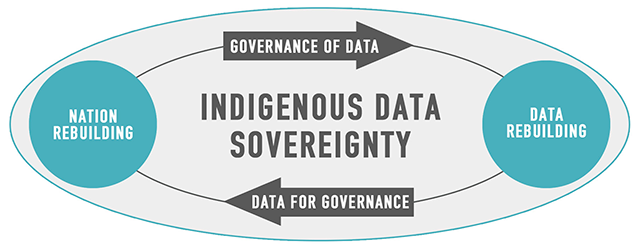
\includegraphics{images/download.png}
\#\#\#\# Info Matters. ``\href{https://open.spotify.com/episode/7lpJvcWPEX0DJcMjQPTdiK?si=r3AfZ-SbQeu3KrMtPbK6cQ}{First Nations data sovereignty}'. August 2021. \{-\}

Info Matters is a podcast by the Information and Privacy Commissioner of Ontario, Canada, Patricia Kosseim. In this episode, Kosseim interviews Dr.~Jonathan Dewer, Chief Executive Officer of the First Nations Information Governance Center, and Carmen Jones, Director of Research and Data Management for the Chief of Ontario. Dewar and Jones provide unique insight into data sovereignty broadly and specifically the creation and implementation of OCAP Principals (14:15).

\hypertarget{guidelines-for-working-with-indigenous-nations}{%
\section{Guidelines for Working With Indigenous Nations}\label{guidelines-for-working-with-indigenous-nations}}

\hypertarget{the-care-principles-for-indigenous-data-governance-care-2020}{%
\subsubsection*{\texorpdfstring{The CARE Principles for Indigenous Data Governance (\href{http://doi.org/10.5334/dsj-2020-043}{CARE}) \textbar{} 2020}{The CARE Principles for Indigenous Data Governance (CARE) \textbar{} 2020}}\label{the-care-principles-for-indigenous-data-governance-care-2020}}
\addcontentsline{toc}{subsubsection}{The CARE Principles for Indigenous Data Governance (\href{http://doi.org/10.5334/dsj-2020-043}{CARE}) \textbar{} 2020}

Carroll, S.R., Garba, I., Figueroa-Rodríguez, O.L., Holbrook, J., Lovett, R., Materechera, S., Parsons, M., Raseroka, K., Rodriguez-Lonebear, D., Rowe, R., Sara, R., Walker, J.D., Anderson, J. and Hudson, M., 2020. The CARE Principles for Indigenous Data Governance. Data Science Journal, 19(1), p.43. \href{http://doi.org/10.5334/dsj-2020-043}{DOI}
The `CARE Principles for Indigenous Data Governance' (Collective Benefit, Authority to Control, Responsibility, and Ethics) were developed due to concerns about secondary use of data and limited opportunities for benefit-sharing between Indigenous communities and outside researchers. While the FAIR Principles are data-centric, the CARE Principles are people and purpose oriented. The authors write, ``the goal is that stewards and other users of Indigenous data will `Be FAIR and CARE.'\,'' CARE principles are intended to be used in concert with FAIR Principals. Of particular note, this paper also provides an important background on Indigenous data sovereignty.

\begin{figure}
\centering
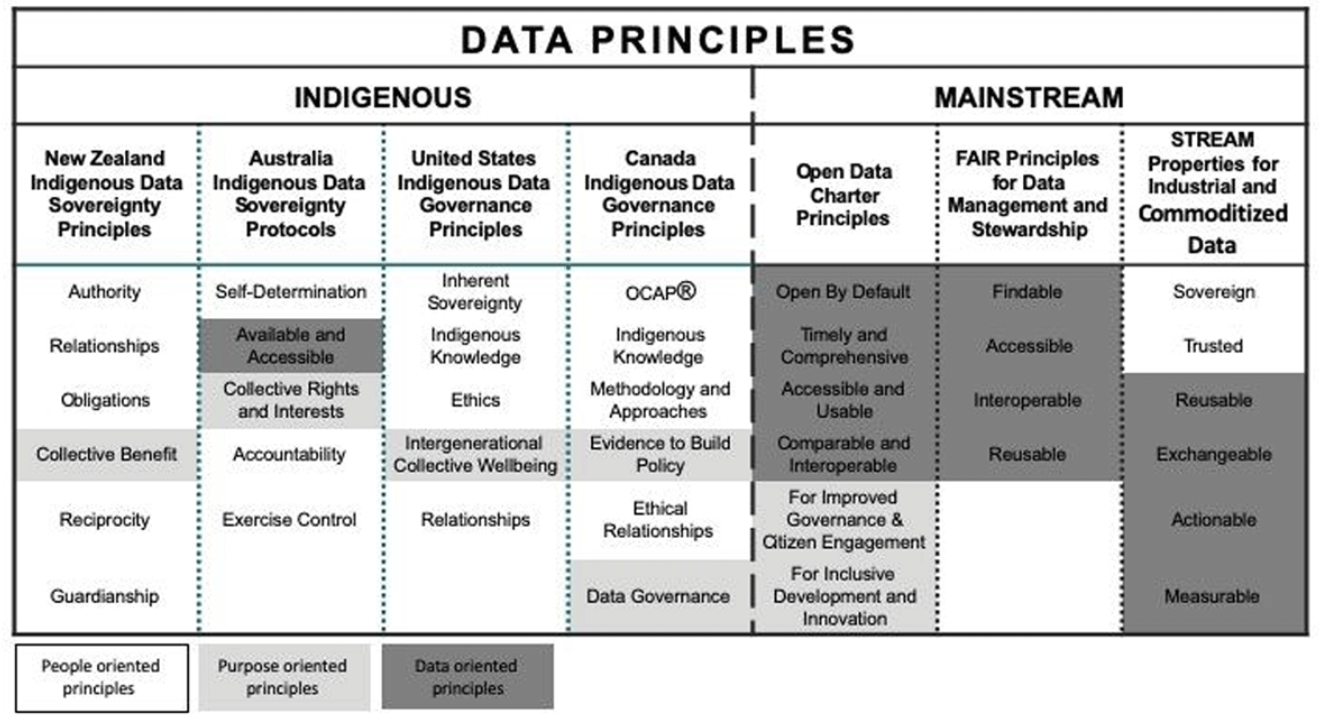
\includegraphics{images/care.png}
\caption{\label{fig:unnamed-chunk-5}Indigenous and mainstream data principles, and the orientation of these principles towards data, people and purpose (Carroll et al.~2020).}
\end{figure}

\hypertarget{ocap-principals}{%
\subsection{OCAP Principals}\label{ocap-principals}}

\hypertarget{ocap---first-nations-ownership-control-access-and-possession-or-self-determination-applied-to-research-2004}{%
\subsubsection*{\texorpdfstring{\href{https://biblio.uottawa.ca/sites/biblio.uottawa.ca/files/bestpractices_fnigc_ocap_fact_sheet_en_final.pdf}{OCAP} - First Nations Ownership, Control, Access and Possession or Self Determination Applied to Research (2004)}{OCAP - First Nations Ownership, Control, Access and Possession or Self Determination Applied to Research (2004)}}\label{ocap---first-nations-ownership-control-access-and-possession-or-self-determination-applied-to-research-2004}}
\addcontentsline{toc}{subsubsection}{\href{https://biblio.uottawa.ca/sites/biblio.uottawa.ca/files/bestpractices_fnigc_ocap_fact_sheet_en_final.pdf}{OCAP} - First Nations Ownership, Control, Access and Possession or Self Determination Applied to Research (2004)}

The OCAP Principals were first developed in 1998 in response to extractive research practices. ``These principals establish how First Nations' data, information, and cultural knowledge should be collected, accessed, used, and shared.''

\hypertarget{fundamentals-of-ocap-course}{%
\subsubsection*{\texorpdfstring{\href{https://fnigc.ca/ocap-training/take-the-course/}{Fundamentals of OCAP Course}}{Fundamentals of OCAP Course}}\label{fundamentals-of-ocap-course}}
\addcontentsline{toc}{subsubsection}{\href{https://fnigc.ca/ocap-training/take-the-course/}{Fundamentals of OCAP Course}}

An online training course to introduce individuals to the fundamental concepts of OCAP, information governance, and First Nations Data Sovereignty.

\hypertarget{data-management-tools}{%
\chapter{Data Management Tools}\label{data-management-tools}}

Thus far, the data management tools we've come across have largely been developed by \href{https://localcontexts.org/labels/biocultural-labels/}{Local Contexts}. If you have examples of other practical tools or organizations that develop them, please share!

\hypertarget{biocultural-labels}{%
\section{Biocultural Labels}\label{biocultural-labels}}

Data labels are text elements that describe individual data points. They are used on metadata as a tag that can be easily categorized and searched. Biocultural (BC) labels are data-markers being piloted by the \href{https://www.enrich-hub.org/bc-labels}{The Biocultural Label Initiative} to help define community expectations and consent about research data use. ``The BC Labels provide a practical application of Indigenous data sovereignty principles to issues of access and benefit-sharing for genetic resources and support Nagoya Protocol expectations around the disclosure and origins of Indigenous data used in research contexts.'' (Anderson \& Hudson 2021)

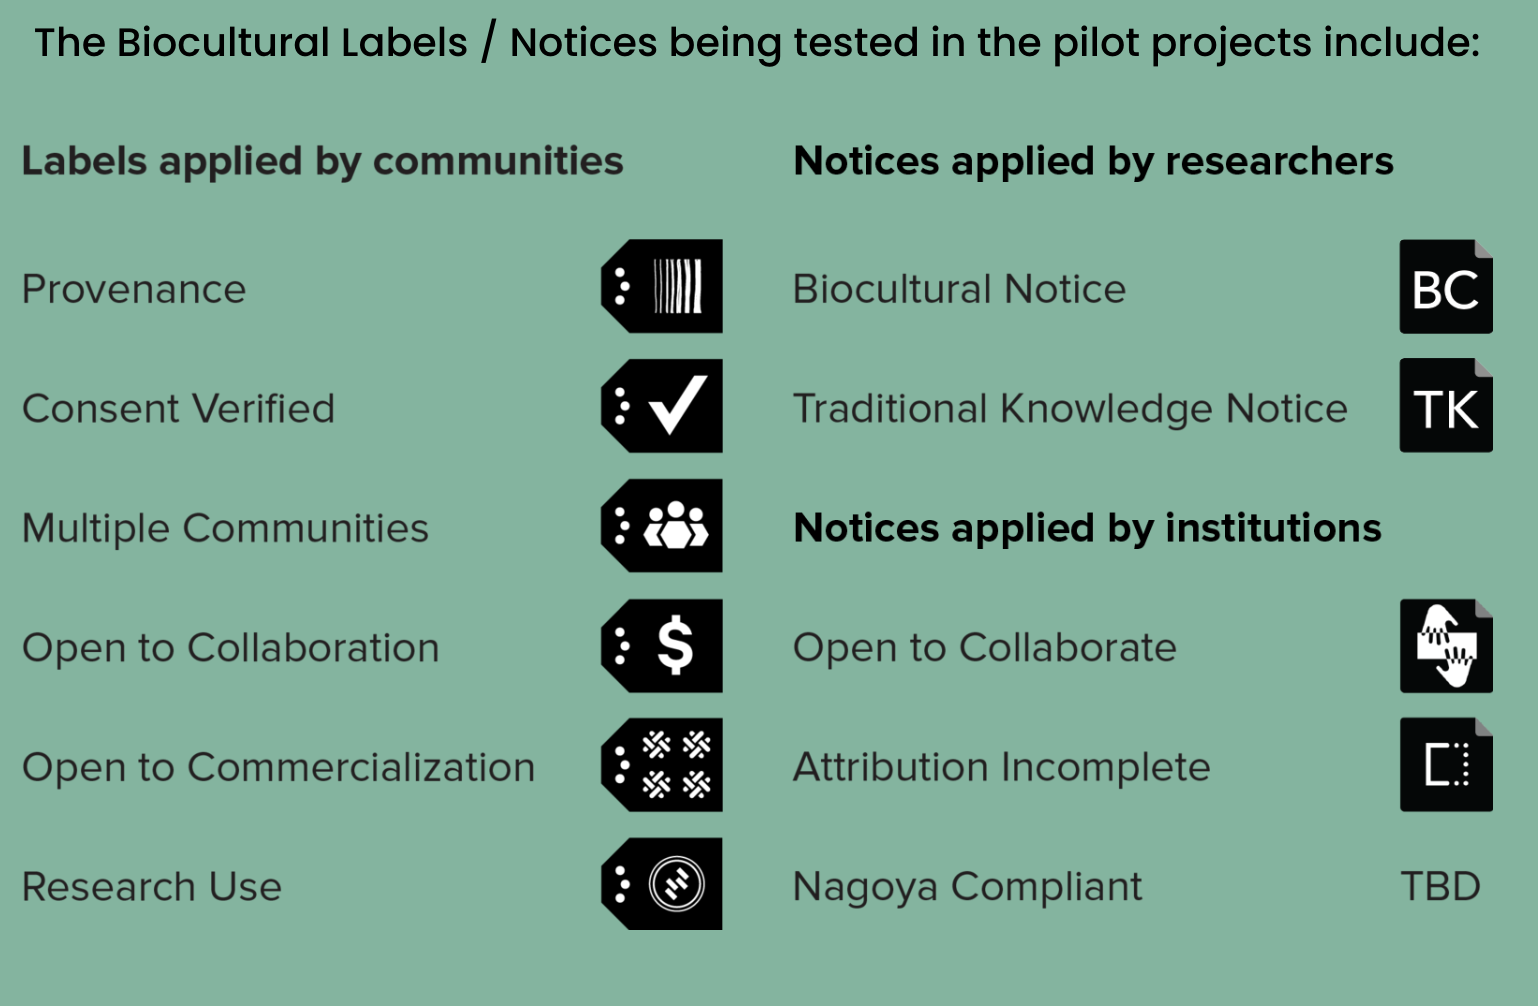
\includegraphics{images/biocultural_labels.png}

\hypertarget{anderson-jane-and-maui-hudson.-stem-inclusive-teaching-practices-webinar-series-the-biocultural-labels-initiative.-2021.}{%
\subsubsection*{\texorpdfstring{Anderson, Jane, and Maui Hudson. ``\href{https://qubeshub.org/publications/2326/1}{STEM Inclusive Teaching Practices Webinar Series}: The Biocultural Labels Initiative.'' (2021).}{Anderson, Jane, and Maui Hudson. ``STEM Inclusive Teaching Practices Webinar Series: The Biocultural Labels Initiative.'' (2021).}}\label{anderson-jane-and-maui-hudson.-stem-inclusive-teaching-practices-webinar-series-the-biocultural-labels-initiative.-2021.}}
\addcontentsline{toc}{subsubsection}{Anderson, Jane, and Maui Hudson. ``\href{https://qubeshub.org/publications/2326/1}{STEM Inclusive Teaching Practices Webinar Series}: The Biocultural Labels Initiative.'' (2021).}

\hypertarget{indigenous-digitial-strategies}{%
\section{Indigenous Digitial Strategies}\label{indigenous-digitial-strategies}}

\hypertarget{local-contexts}{%
\subsubsection*{\texorpdfstring{\href{https://localcontexts.org/labels/biocultural-labels/}{Local Contexts}}{Local Contexts}}\label{local-contexts}}
\addcontentsline{toc}{subsubsection}{\href{https://localcontexts.org/labels/biocultural-labels/}{Local Contexts}}

Local Contexts is an organization that offers digital strategies for Indigenous communities, cultural institutions and researchers through Traditional Knowledge and Biocultural Labels and Notices and licenses for intellectual property.

\hypertarget{open-data-principals}{%
\chapter{Open Data Principals}\label{open-data-principals}}

The Open Data movement has had significant success. Data is more accessible than ever before. The Findable, Accessible, Interoperable and Reusable (FAIR) Data Principles were developed to improve the reuse of scholarly data. However, data collection, analysis and sharing is couched in historic inequities. The FAIR principles, now paired with CARE, can work together to ensure data is ethically sourced and shared.

\hypertarget{fair-principals}{%
\subsection{FAIR Principals}\label{fair-principals}}

\hypertarget{wilkinson-mark-d.-et-al.-the-fair-guiding-principles-for-scientific-data-management-and-stewardship.-scientific-data-3.1-2016-1-9.}{%
\subsubsection*{\texorpdfstring{Wilkinson, Mark D., et al.~``\href{https://www.nature.com/articles/sdata201618}{The FAIR Guiding Principles for scientific data management and stewardship}.'' Scientific Data 3.1 (2016): 1-9.}{Wilkinson, Mark D., et al.~``The FAIR Guiding Principles for scientific data management and stewardship.'' Scientific Data 3.1 (2016): 1-9.}}\label{wilkinson-mark-d.-et-al.-the-fair-guiding-principles-for-scientific-data-management-and-stewardship.-scientific-data-3.1-2016-1-9.}}
\addcontentsline{toc}{subsubsection}{Wilkinson, Mark D., et al.~``\href{https://www.nature.com/articles/sdata201618}{The FAIR Guiding Principles for scientific data management and stewardship}.'' Scientific Data 3.1 (2016): 1-9.}

The Findable, Accessible, Interoperable and Reusable (FAIR) Data principles were developed in reaction to the wide reuse of scholarly data. They have become increasingly important, acting as guidelines to improve the entire lifecycle of research data management (D7.4 2021). The term ``FAIR'' was first developed at a Lorentz workshop in the Netherlands in 2014 (D7.4 2021).

\hypertarget{boeckhout-martin-gerhard-a.-zielhuis-and-annelien-l.-bredenoord.-the-fair-guiding-principles-for-data-stewardship-fair-enough.-european-journal-of-human-genetics-26.7-2018-931-936.}{%
\subsubsection*{\texorpdfstring{Boeckhout, Martin, Gerhard A. Zielhuis, and Annelien L. Bredenoord. ``\href{https://www.ncbi.nlm.nih.gov/pmc/articles/PMC6018669/}{The FAIR guiding principles for data stewardship: fair enough?}.'' European Journal of Human Genetics 26.7 (2018): 931-936.}{Boeckhout, Martin, Gerhard A. Zielhuis, and Annelien L. Bredenoord. ``The FAIR guiding principles for data stewardship: fair enough?.'' European Journal of Human Genetics 26.7 (2018): 931-936.}}\label{boeckhout-martin-gerhard-a.-zielhuis-and-annelien-l.-bredenoord.-the-fair-guiding-principles-for-data-stewardship-fair-enough.-european-journal-of-human-genetics-26.7-2018-931-936.}}
\addcontentsline{toc}{subsubsection}{Boeckhout, Martin, Gerhard A. Zielhuis, and Annelien L. Bredenoord. ``\href{https://www.ncbi.nlm.nih.gov/pmc/articles/PMC6018669/}{The FAIR guiding principles for data stewardship: fair enough?}.'' European Journal of Human Genetics 26.7 (2018): 931-936.}

\hypertarget{d7.4-how-to-be-fair-with-your-data.-a-teaching-and-training-handbook-for-higher-education-institutions.-november-2021.}{%
\subsubsection*{\texorpdfstring{D7.4 \href{https://zenodo.org/record/5837500\#.Yhk8L5PMJ6e}{How to be FAIR with your data}. A teaching and training handbook for higher education institutions. November 2021.}{D7.4 How to be FAIR with your data. A teaching and training handbook for higher education institutions. November 2021.}}\label{d7.4-how-to-be-fair-with-your-data.-a-teaching-and-training-handbook-for-higher-education-institutions.-november-2021.}}
\addcontentsline{toc}{subsubsection}{D7.4 \href{https://zenodo.org/record/5837500\#.Yhk8L5PMJ6e}{How to be FAIR with your data}. A teaching and training handbook for higher education institutions. November 2021.}

The handbook was written and edited by a group of about 40 collaborators as part of a working group and was subject to community review. The 179 page book is a wealth of information and practical materials relating to the FAIR principals. Practical materials include competence profiles, learning outcomes and lesson plans, and supporting information.

\hypertarget{fair-and-beyond}{%
\subsection{FAIR and Beyond}\label{fair-and-beyond}}

For CARE Principals, see Section 3.3: Guidelines for Working With Indigenous Nations

\hypertarget{austin-claire-c.-et-al.-fostering-global-data-sharing-highlighting-the-recommendations-of-the-research-data-alliance-covid-19-working-group.-wellcome-open-research-5-2020.}{%
\subsubsection*{\texorpdfstring{Austin, Claire C., et al.~``\href{https://www.ncbi.nlm.nih.gov/pmc/articles/PMC7808050/}{Fostering global data sharing: highlighting the recommendations of the Research Data Alliance COVID-19 working group.}'' Wellcome Open Research 5 (2020).}{Austin, Claire C., et al.~``Fostering global data sharing: highlighting the recommendations of the Research Data Alliance COVID-19 working group.'' Wellcome Open Research 5 (2020).}}\label{austin-claire-c.-et-al.-fostering-global-data-sharing-highlighting-the-recommendations-of-the-research-data-alliance-covid-19-working-group.-wellcome-open-research-5-2020.}}
\addcontentsline{toc}{subsubsection}{Austin, Claire C., et al.~``\href{https://www.ncbi.nlm.nih.gov/pmc/articles/PMC7808050/}{Fostering global data sharing: highlighting the recommendations of the Research Data Alliance COVID-19 working group.}'' Wellcome Open Research 5 (2020).}

This letter, developed by a 160 person international working group, shares a set of recommendations and guidelines on data sharing and best practices for COVID-19 research. Here, the authors create recommendations that balance adherence to FAIR Principles but given the nature of COVID-19, also need quick data release.

\hypertarget{boeckhout-martin-gerhard-a.-zielhuis-and-annelien-l.-bredenoord.-the-fair-guiding-principles-for-data-stewardship-fair-enough.-european-journal-of-human-genetics-26.7-2018-931-936.-1}{%
\subsubsection*{\texorpdfstring{Boeckhout, Martin, Gerhard A. Zielhuis, and Annelien L. Bredenoord. ``\href{https://www.ncbi.nlm.nih.gov/pmc/articles/PMC6018669/}{The FAIR guiding principles for data stewardship: fair enough?.}'' European Journal of Human Genetics 26.7 (2018): 931-936.}{Boeckhout, Martin, Gerhard A. Zielhuis, and Annelien L. Bredenoord. ``The FAIR guiding principles for data stewardship: fair enough?.'' European Journal of Human Genetics 26.7 (2018): 931-936.}}\label{boeckhout-martin-gerhard-a.-zielhuis-and-annelien-l.-bredenoord.-the-fair-guiding-principles-for-data-stewardship-fair-enough.-european-journal-of-human-genetics-26.7-2018-931-936.-1}}
\addcontentsline{toc}{subsubsection}{Boeckhout, Martin, Gerhard A. Zielhuis, and Annelien L. Bredenoord. ``\href{https://www.ncbi.nlm.nih.gov/pmc/articles/PMC6018669/}{The FAIR guiding principles for data stewardship: fair enough?.}'' European Journal of Human Genetics 26.7 (2018): 931-936.}

\hypertarget{examples-of-indigenous-environmental-synthesis-and-data-science}{%
\chapter{Examples of Indigenous Environmental Synthesis and Data Science}\label{examples-of-indigenous-environmental-synthesis-and-data-science}}

\hypertarget{environmental-synthesis}{%
\section{Environmental Synthesis}\label{environmental-synthesis}}

\hypertarget{garnett-stephen-t.-et-al.-a-spatial-overview-of-the-global-importance-of-indigenous-lands-for-conservation.-nature-sustainability-1.7-2018-369-374.}{%
\subsubsection*{\texorpdfstring{Garnett, Stephen T., et al.~``\href{https://www.nature.com/articles/s41893-018-0100-6?ss_source=sscampaigns\&ss_campaign_id=5c424fe9d20e280001eb02bf\&ss_email_id=5c5cf4c39bca21000175c9fd\&ss_campaign_name=Introducing+the+Interfaith+Rainforest+Initiative\&ss_campaign_sent_date=2019-02-08T03:17:24Z}{A spatial overview of the global importance of Indigenous lands for conservation}.'' Nature Sustainability 1.7 (2018): 369-374.}{Garnett, Stephen T., et al.~``A spatial overview of the global importance of Indigenous lands for conservation.'' Nature Sustainability 1.7 (2018): 369-374.}}\label{garnett-stephen-t.-et-al.-a-spatial-overview-of-the-global-importance-of-indigenous-lands-for-conservation.-nature-sustainability-1.7-2018-369-374.}}
\addcontentsline{toc}{subsubsection}{Garnett, Stephen T., et al.~``\href{https://www.nature.com/articles/s41893-018-0100-6?ss_source=sscampaigns\&ss_campaign_id=5c424fe9d20e280001eb02bf\&ss_email_id=5c5cf4c39bca21000175c9fd\&ss_campaign_name=Introducing+the+Interfaith+Rainforest+Initiative\&ss_campaign_sent_date=2019-02-08T03:17:24Z}{A spatial overview of the global importance of Indigenous lands for conservation}.'' Nature Sustainability 1.7 (2018): 369-374.}

This paper provides the first global assessment of global lands within Indigenous stewardship and it's overlap with protected areas and conservation outcomes. The authors found that Indigenous Peoples have tenure rights or actively manage more than a quarter of the world's land surface (\textasciitilde38 million km\textsuperscript{2} across 87 countries). Indigenous managed lands account for about 40\% of all terrestrial protected areas and ecologically intact landscapes (for example, boreal and tropical primary forests, savannas and marshes). Thus, indigenous stewarded lands are critical hubs for biodiversity and resilience.

To create this global assessment, the authors rely on 127 publicly available data sources, including real estate (cadastral) records for state-recognized Indigenous Peoples' lands, publicly accessible participatory mapping, models based on census data and maps derived from scholarly publications. Here, the authors worked to overcome some of the inherent biases in Indigenous geospatial data. Data of Indigenous Peoples' land occupation or management tend to rely on state-sanctioned data that can be deployed to disenfranchise Indigenous Peoples (\href{https://www.sciencedirect.com/science/article/pii/S0016718510001090?via\%3Dihub}{Bryan 2011}; Garnett et al.~2018). The authors write, ``the dearth of reliable data on Indigenous Peoples' lands in many parts of the world has implications not only for securing their rights but also for the conservation and management of a significant proportion of terrestrial global biodiversity.''

\begin{figure}
\centering
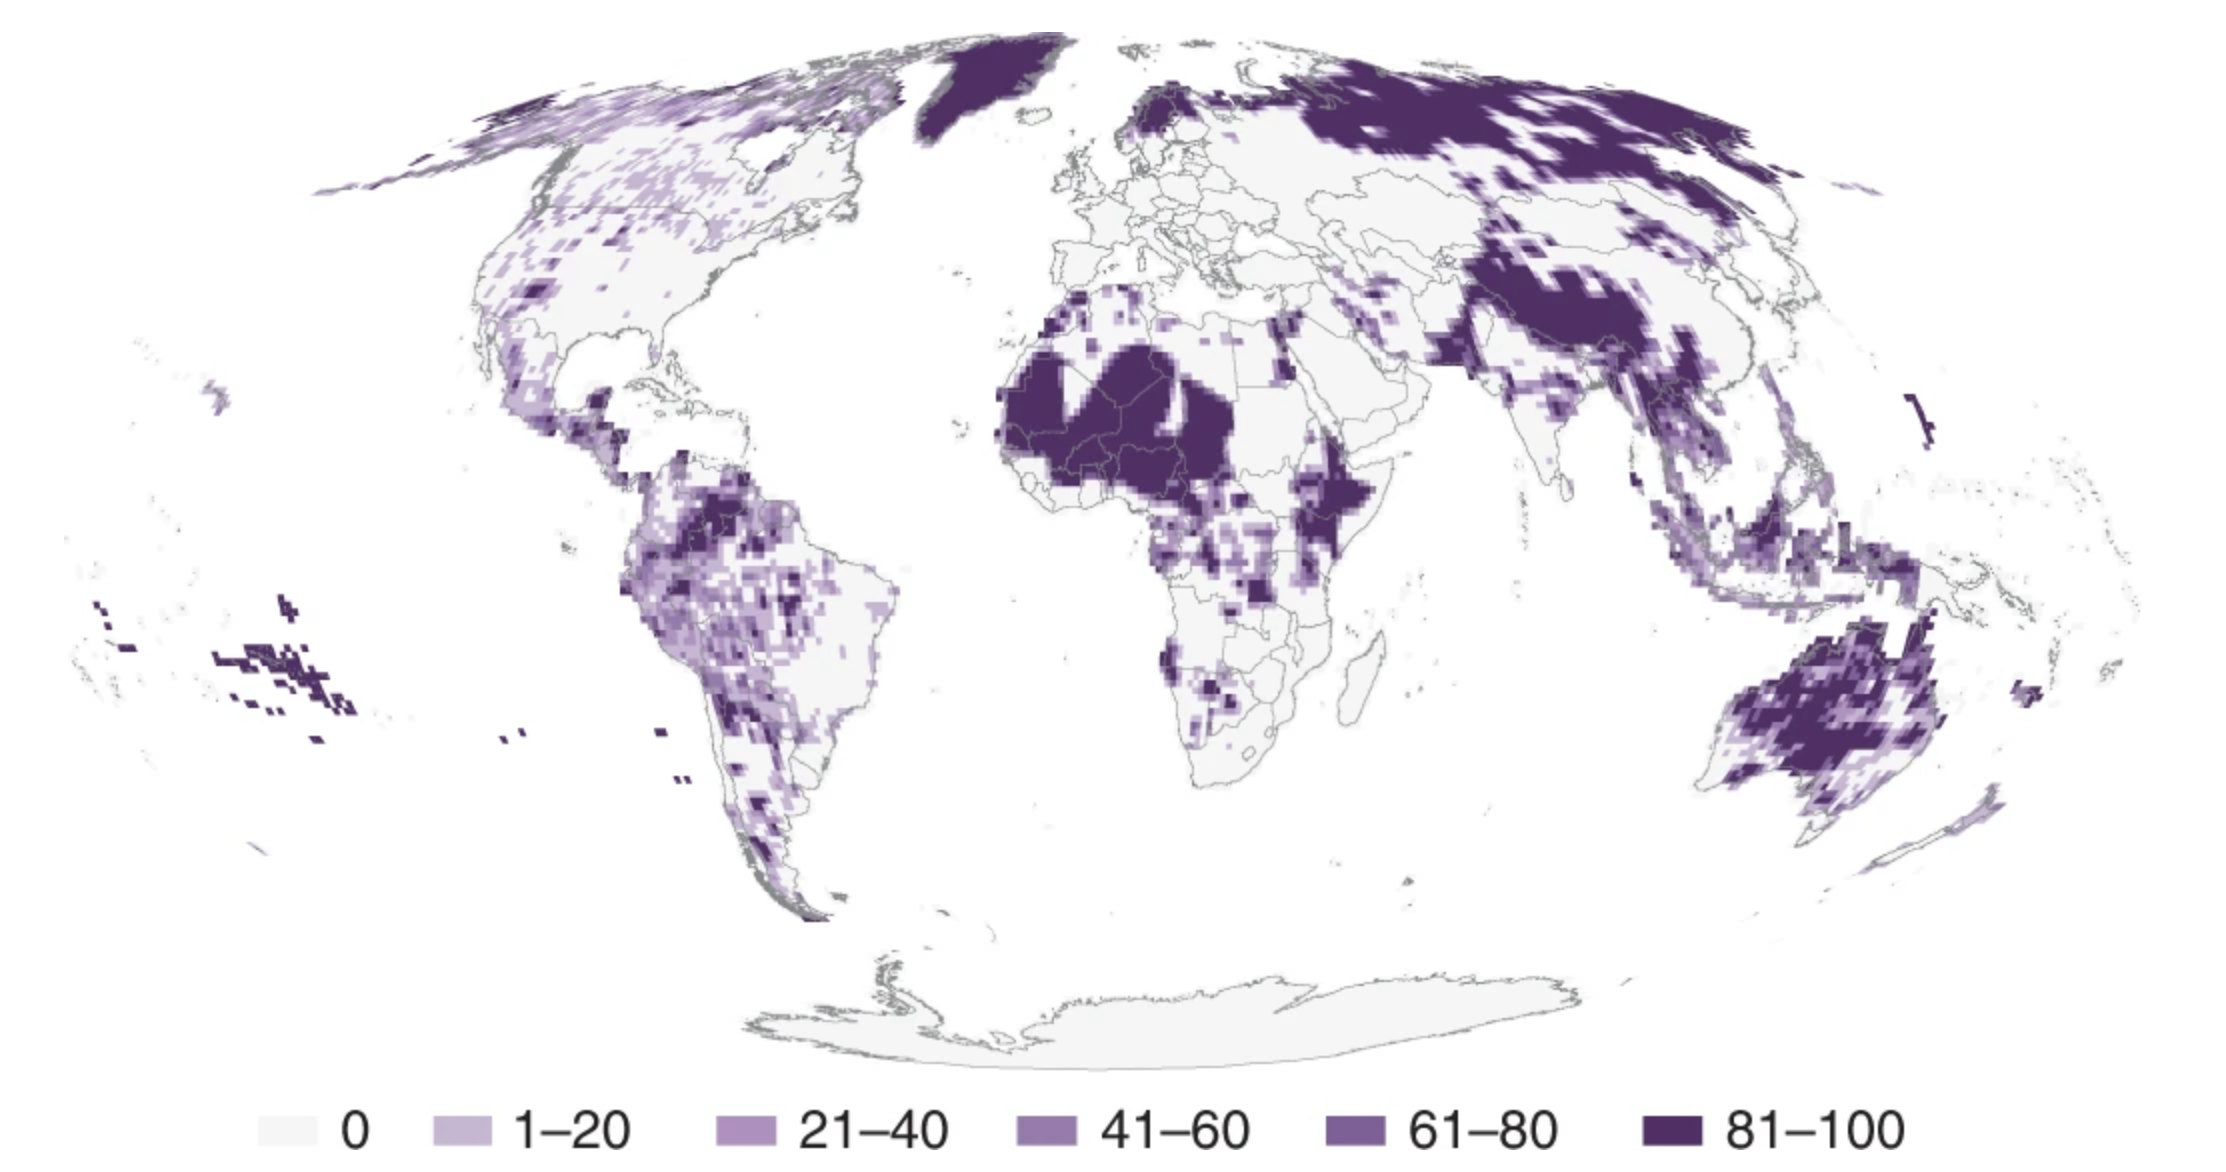
\includegraphics{images/Garnett_2018.png}
\caption{\label{fig:unnamed-chunk-7}Global map of lands managed or controlled by Indigengous Peoples. Purple shading represents the percentage of each degree square mapped as Indigenous in at least one of 127 source documents. Blank areas do not neccesarily indicate an absence of Indigenous Peoples or lands (Garnett et al.~2018).}
\end{figure}

\hypertarget{indigenous-environmental-data}{%
\section{Indigenous Environmental Data}\label{indigenous-environmental-data}}

\hypertarget{warm-regards.-indigenous-climate-knowledge-and-data-sovereignty.-february-2021.}{%
\subsubsection*{\texorpdfstring{Warm Regards. ``\href{https://open.spotify.com/episode/4Gdp1RSChCPM0qftRun3DD?si=pcVeYiwwQIWnlKynt4-ADQ}{Indigenous Climate Knowledge and Data Sovereignty}.'' February 2021.}{Warm Regards. ``Indigenous Climate Knowledge and Data Sovereignty.'' February 2021.}}\label{warm-regards.-indigenous-climate-knowledge-and-data-sovereignty.-february-2021.}}
\addcontentsline{toc}{subsubsection}{Warm Regards. ``\href{https://open.spotify.com/episode/4Gdp1RSChCPM0qftRun3DD?si=pcVeYiwwQIWnlKynt4-ADQ}{Indigenous Climate Knowledge and Data Sovereignty}.'' February 2021.}

Warm Regards is a podcast about life on a warming planet. In this episode, the hosts interview two Indigenous scientists, James Rattling Leaf, Sr.~and Krystal Tsosie, about traditional ecological knowledges and data sovereignty.

\hypertarget{traditional-ecological-knowledge-tek}{%
\section{Traditional Ecological Knowledge (TEK)}\label{traditional-ecological-knowledge-tek}}

Below are a couple examples which speak to how TEK and other forms of knowledge, such as western science, can work together to increase understanding and improve land stewardship.

\hypertarget{reid-andrea.-learning-from-indigenous-knowledge-holders-on-the-state-and-future-of-wild-pacific-salmon.-the-conversation.-may-2022.}{%
\subsubsection*{\texorpdfstring{Reid, Andrea. ``\href{https://theconversation.com/learning-from-indigenous-knowledge-holders-on-the-state-and-future-of-wild-pacific-salmon-182411}{Learning from Indigenous knowledge holders on the state and future of wild Pacific salmon}.'' The Conversation. May 2022.}{Reid, Andrea. ``Learning from Indigenous knowledge holders on the state and future of wild Pacific salmon.'' The Conversation. May 2022.}}\label{reid-andrea.-learning-from-indigenous-knowledge-holders-on-the-state-and-future-of-wild-pacific-salmon.-the-conversation.-may-2022.}}
\addcontentsline{toc}{subsubsection}{Reid, Andrea. ``\href{https://theconversation.com/learning-from-indigenous-knowledge-holders-on-the-state-and-future-of-wild-pacific-salmon-182411}{Learning from Indigenous knowledge holders on the state and future of wild Pacific salmon}.'' The Conversation. May 2022.}

Andrea Reid, a member of the Nisga'a Nation and Director for the Centre of Indigenous Fisheries at University of British Columbia, writes about her experience working with Nisga'a Nation tribal elders to understand threats to salmon. She provides an overview of the issues with much of western science's approach when working with TEK and explains her current research in a brief narrative. For scholarly examples of Indigenous fisheries science, see Dr.~Reid's \href{https://scholar.google.com/citations?hl=en\&user=WWdYxJgAAAAJ}{work}.

\hypertarget{reid-andrea-j.-et-al.-twoeyed-seeing-an-indigenous-framework-to-transform-fisheries-research-and-management.-fish-and-fisheries-22.2-2021-243-261.}{%
\subsubsection*{\texorpdfstring{Reid, Andrea J., et al.~````\href{https://onlinelibrary.wiley.com/doi/full/10.1111/faf.12516}{Two‐Eyed Seeing'': An Indigenous framework to transform fisheries research and management}.'' Fish and Fisheries 22.2 (2021): 243-261.}{Reid, Andrea J., et al.~``\,``Two‐Eyed Seeing'': An Indigenous framework to transform fisheries research and management.'' Fish and Fisheries 22.2 (2021): 243-261.}}\label{reid-andrea-j.-et-al.-twoeyed-seeing-an-indigenous-framework-to-transform-fisheries-research-and-management.-fish-and-fisheries-22.2-2021-243-261.}}
\addcontentsline{toc}{subsubsection}{Reid, Andrea J., et al.~````\href{https://onlinelibrary.wiley.com/doi/full/10.1111/faf.12516}{Two‐Eyed Seeing'': An Indigenous framework to transform fisheries research and management}.'' Fish and Fisheries 22.2 (2021): 243-261.}

Highly relevant to current shifts in ecosystem management, Reid et al.~(2021) suggests a framework, Two-Eyed Seeing, in order to understand and steward fisheries. Rather than assimilating Indigenous knowledge systems into western science, Two-Eyed Seeing embraces ``learning to see from one eye with the strengths of Indigenous knowledges and ways of knowing, and from the other eye with the strengths of mainstream knowledges and ways of knowing, and to use both these eyes together, for the benefit of all'' (Elder Dr.~Albert Marshall; Reid et al.~2021).
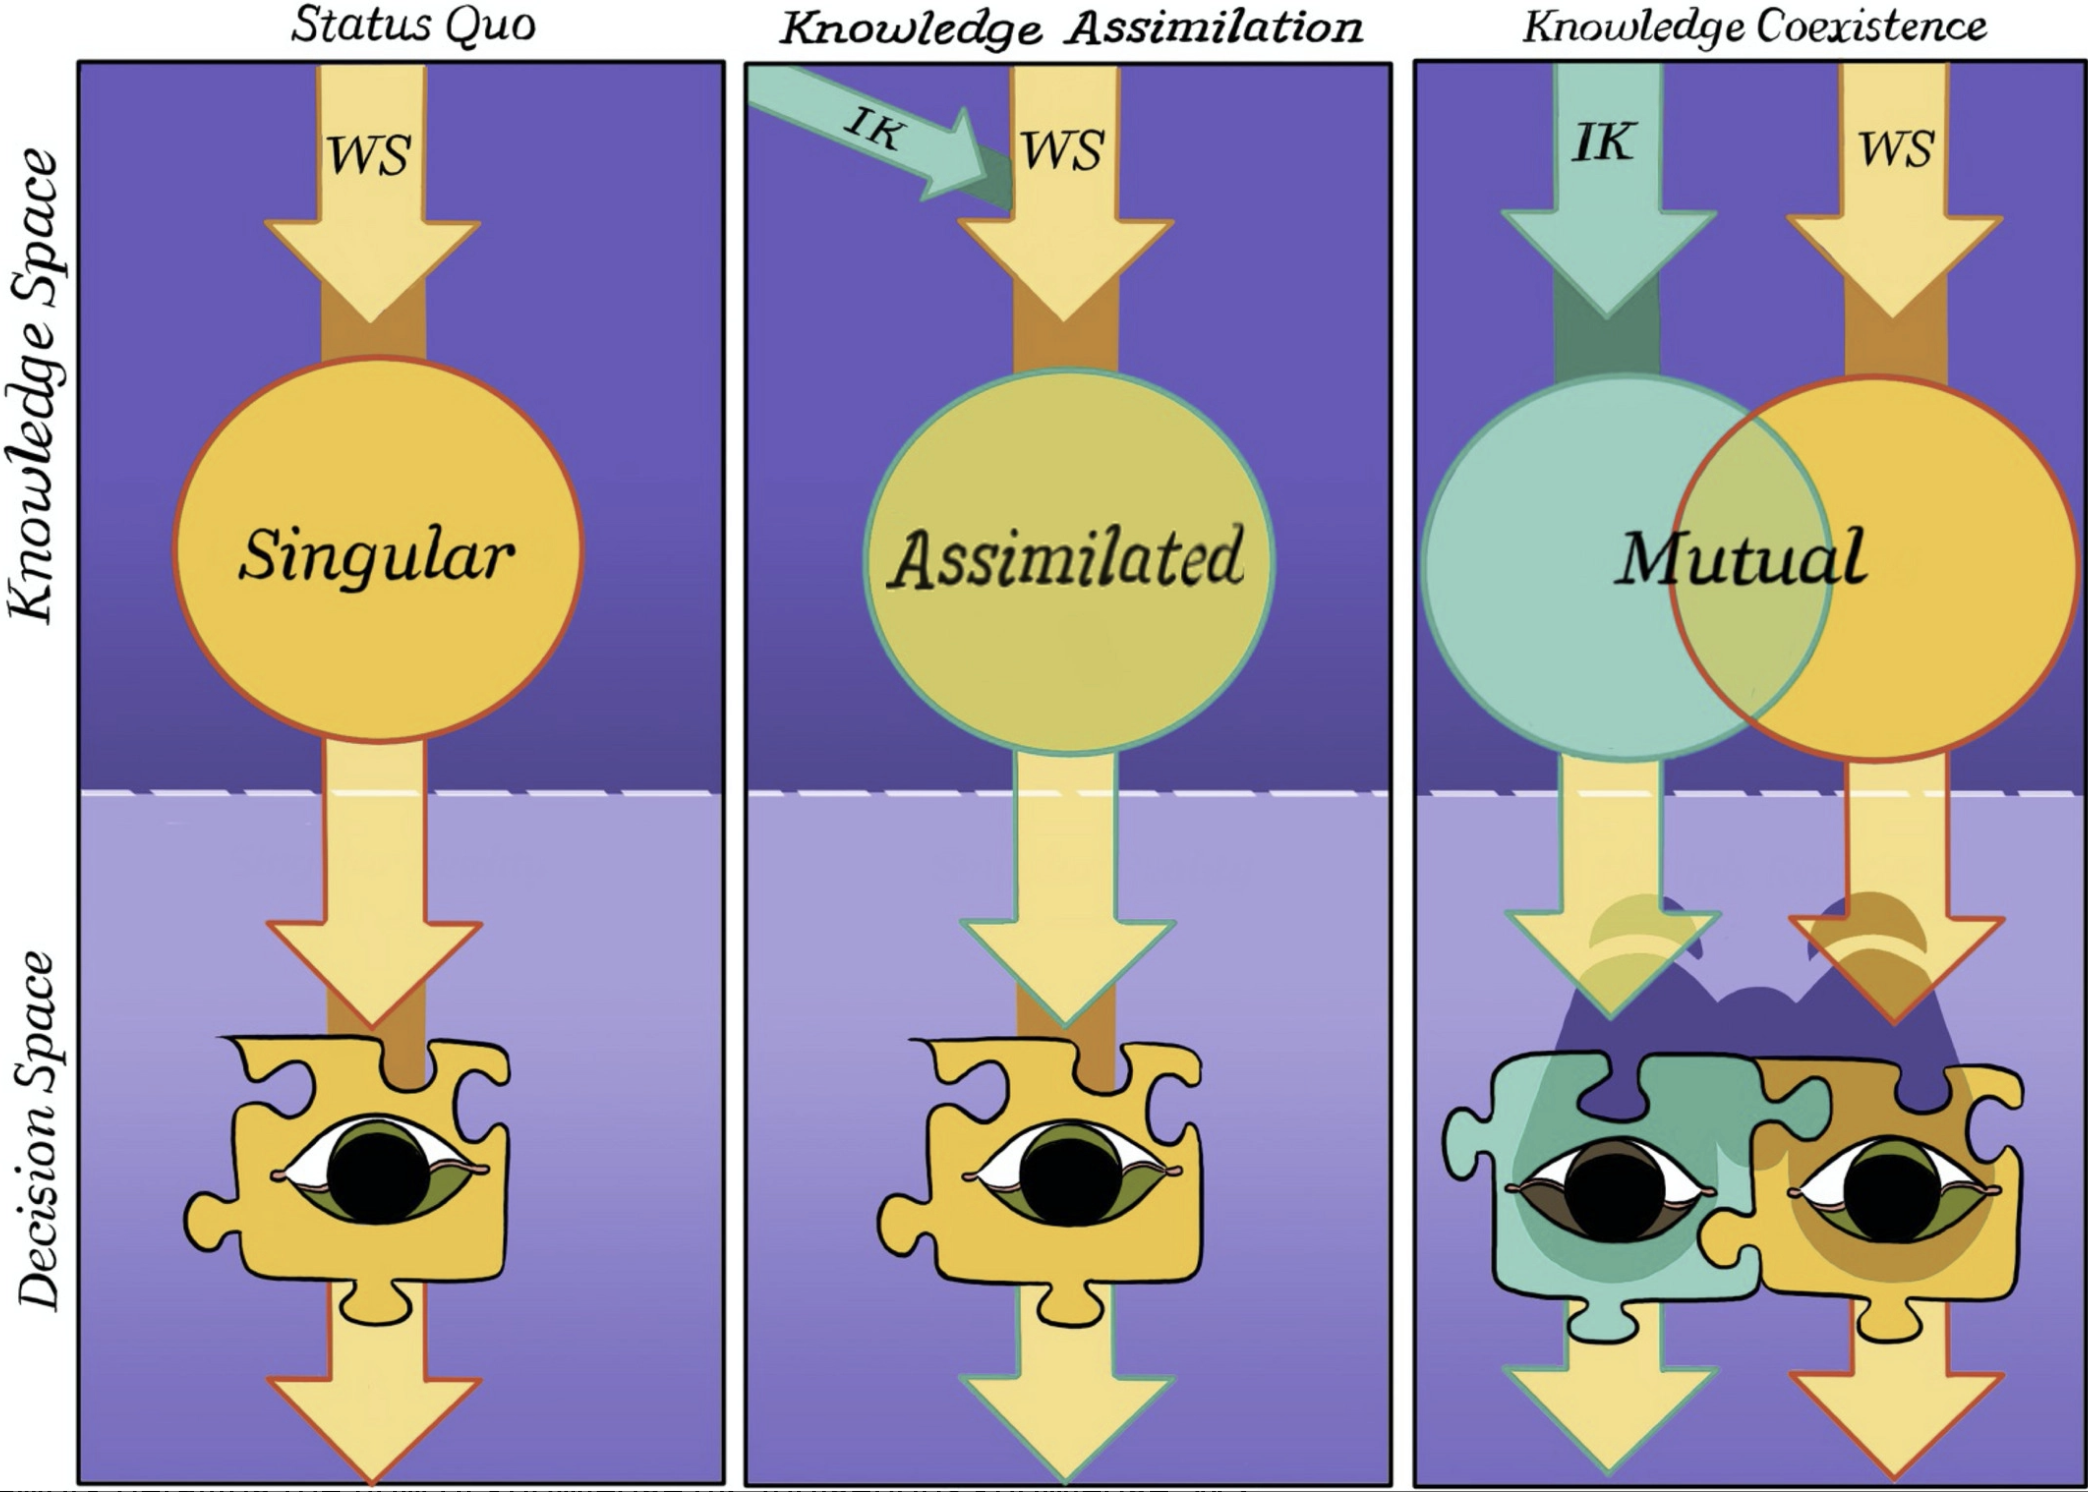
\includegraphics{images/Reid_2021.png}

Bryan, J. Walking the line: participatory mapping, Indigenous rights, and neoliberalism. Geoforum 42, 40--50 (2011). \url{https://www.sciencedirect.com/science/article/pii/S0016718510001090?via\%3Dihub}

Walter, M, Lovett, R, Bodkin Andrews, G and Lee, V. 2018. Indigenous Data Sovereignty Briefing Paper 1. Miaim nayri Wingara Data Sovereignty Group and the Australian Indigenous Governance Institute. We acknowledge the pioneering contribution of John Taylor.

  \bibliography{book.bib,packages.bib}

\end{document}
